\documentclass[letterpaper]{article}
\usepackage{aaai24}
\usepackage{times}
\usepackage{helvet}
\usepackage{courier}
\usepackage[hidelinks]{hyperref}
\usepackage{amsmath,amssymb,amsfonts}
\usepackage{graphicx}
\usepackage{booktabs}
\usepackage{microtype}
\usepackage{cite}

\title{The Algorithmic Monoculture Paradox: Simulating Epistemic Degradation in Foundation-Model-Mediated Social Networks}

% ---------------------------------------------------------------------------
% AUTHOR BLOCK: PREPRINT VERSION 2 (FOR ZENODO ARCHIVE)
% DOI: 10.5281/zenodo.23836280
% ---------------------------------------------------------------------------
\author{
    \textbf{Ashuraj Herode}\textsuperscript{\rm 1}\thanks{Corresponding author: herodeashuraj@gmail.com},
    \textbf{Dr. Prakash Parmar}\textsuperscript{\rm 1}
}
\affiliations{
    \textsuperscript{\rm 1}Department of Computer Engineering, Vidyalankar Institute of Technology, University of Mumbai, India\\
    \texttt{herodeashuraj@gmail.com}, \texttt{prakash.parmar@vit.edu.in}
}

\begin{document}

\maketitle

\begin{abstract}
The ``Wisdom of Crowds'' principle demonstrates that distributed groups of imperfect decision-makers can achieve superior collective accuracy because independent, idiosyncratic errors cancel out upon aggregation. Today, the rapid integration of centralized foundation models (LLMs) into decision-making workflows threatens the epistemic independence that underlies this dynamic. When independent human agents query shared foundation models, individual error variance is suppressed, replacing independent noise with shared, correlated algorithmic bias. Here, we investigate this phenomenon by formalizing a discrete-event network simulation combining Scott Page's Diversity Prediction Theorem with an iterated DeGroot consensus framework across macro-scale social graphs ($N = 1,000$ agents). Across 2,970 Monte Carlo simulations spanning three canonical network topologies (Watts-Strogatz Small-World, Barabási-Albert Scale-Free, and Erd\H{o}s-R\'enyi Random) and three correlation regimes, we show that high reliance on a centralized foundation model ($\rho = 0.90$) causes Collective Squared Error to escalate by over $+16$ squared error units (a 29- to 82-fold increase depending on network topology, with an average 50-fold escalation from a pooled baseline of $0.339 \pm 0.08$ to $16.833 \pm 2.05$). We prove analytically that because uniform external advice passes directly through any row-stochastic network matrix ($\mathbf{W}\mathbf{1}=\mathbf{1}$), the AI-driven error component is strictly topology-invariant and governed by $\mathbb{E}[(c^* - \theta)^2] = \mu_{AI}^2 + \frac{\alpha}{2-\alpha}\rho\sigma_{AI}^2$. Consequently, persistent directional bias ($\mu_{AI}$) is asymptotically absorbed for any reliance $\alpha > 0$ under repeated consultation. Crucially, while an unconstrained polyculture ($\rho = 0.00$) eliminates correlated variance, its collective error remains bounded near the directional bias floor ($3.974 \pm 0.05$)—approximately 12-fold higher than the unassisted crowd. These findings provide an open, runnable computational framework for understanding how individual heuristic reliance under shared generative AI triggers systemic epistemic fragility.
\end{abstract}

\section{Introduction}
For over a century, social epistemology and mathematical statistics have recognized that collective intelligence emerges from cognitive diversity \cite{galton1907vox, page2007difference, lorenz2011social, becker2017network}. In classical human deliberation, whether forecasting economic indices, evaluating scientific hypotheses, or curating public knowledge, individual human agents possess idiosyncratic biases and noisy heuristics. Crucially, when these errors are uncorrelated, aggregation mechanics—such as averaging or consensus formation—cause noise to cancel out, allowing the collective judgment of the crowd to outperform even its most capable individual members.

The rapid, worldwide deployment of generative foundation models (Large Language Models, or LLMs) has disrupted this epistemic architecture. Today, millions of professionals, researchers, students, and autonomous software agents rely on a small handful of centralized foundation models for heuristic guidance, text synthesis, and decision support \cite{bommasani2022opportunities}. 

At the individual level, this technological transition is undeniably advantageous: querying an aligned foundation model reduces individual task completion time, resolves syntactical ambiguities, and frequently lowers individual error relative to uninformed guessing. However, evaluating AI assistance purely at the level of the individual decision-maker commits an ecological fallacy. Inspired by the foundational concept of algorithmic monoculture formalized by Kleinberg and Raghavan \cite{kleinberg2021algorithmic}, when independent entities adopt identical or highly correlated algorithmic decision rules, the system exhibits \textbf{Algorithmic Monoculture}.

Recent audits suggest that aligned foundation models exhibit generative monoculture \cite{wu2025generative}, where post-training alignment constrains output diversity, while behavioral experiments indicate that generative assistance can homogenize creative outputs across human users \cite{doshi2024generative}. 

While existing literature has examined algorithmic monoculture in static selection and ranking tasks \cite{kleinberg2021algorithmic}, the sociotechnical reality of human discourse is fundamentally networked. Humans do not interact with algorithms in isolation; they deliberate, exchange beliefs, and form consensus across structured communication topologies \cite{watts1998collective, barabasi1999emergence, golub2010naive, zollman2007communication}.

This paper addresses a fundamental open question at the intersection of network science, social computing, and AI governance:
\begin{quote}
\textit{How does algorithmic reliance ($\alpha$) alter the epistemic aggregation of a networked crowd, what is the steady-state impact of inter-model correlation ($\rho$), and does network topology buffer or accelerate collective error?}
\end{quote}

Through a macro-scale computational framework encompassing 2,970 Monte Carlo simulations across $1,000$-agent networks, we formalize the interaction between Scott Page's Diversity Prediction Theorem \cite{page2007difference} and iterated DeGroot consensus dynamics \cite{degroot1974reaching, golub2010naive, friedkin1990social}. Our findings demonstrate that algorithmic monoculture acts as an epistemic variance-destroyer, triggering substantial surges in collective error even when individual models appear locally accurate.

\section{Theoretical Framework \& Related Work}

\subsection{The Diversity Prediction Theorem}
Let $\theta \in \mathbb{R}$ represent an objective ground truth parameter. Suppose a crowd of $n$ agents provides estimates $s_1, s_2, \dots, s_n$. The mean collective prediction is defined as $c = \frac{1}{n} \sum_{i=1}^n s_i$. 

Page \cite{page2007difference} (formalizing the ensemble ambiguity decomposition of Krogh and Vedelsby \cite{krogh1995neural}) established that collective squared error can be exactly decomposed into two opposing terms:
\begin{equation}
(c - \theta)^2 = \frac{1}{n} \sum_{i=1}^n (s_i - \theta)^2 - \frac{1}{n} \sum_{i=1}^n (s_i - c)^2
\label{eq:page_theorem}
\end{equation}
which is expressed conceptually as:
\begin{equation}
\mathrm{Error}_{\mathrm{coll}} = \overline{\mathrm{Error}}_{\mathrm{ind}} - \mathrm{Diversity}
\end{equation}

Equation \ref{eq:page_theorem} holds as an exact mathematical identity. Crucially, the minus sign demonstrates that cognitive diversity (the variance of individual estimates around the crowd mean) is a direct mathematical offset against collective error. If an external intervention collapses diversity without a commensurate reduction in individual error, the collective prediction must strictly degrade.

\subsection{Iterated DeGroot Dynamics with External AI Advice}
In an idealized crowd, individual human estimates follow an independent noise model:
\begin{equation}
s_i = \theta + \epsilon_i, \quad \mathbb{E}[\epsilon_i] = 0, \quad \text{Cov}(\epsilon_i, \epsilon_j) = 0 \quad (\forall i \neq j)
\end{equation}
Under independent noise, the variance of the sample mean scales as $\text{Var}(c) = \frac{\sigma^2}{n} \xrightarrow{n \to \infty} 0$. 

Now consider an epistemic network where agents iteratively update beliefs via DeGroot consensus while querying external algorithmic advice, analogous to classical social influence models with forceful external agents \cite{friedkin1990social, acemoglu2010spread}. At each timestep $t$, the belief vector $\mathbf{x}(t) \in \mathbb{R}^N$ evolves according to:
\begin{equation}
\mathbf{x}(t+1) = (1 - \alpha) \mathbf{W} \mathbf{x}(t) + \alpha \hat{\boldsymbol{\theta}}_M(t)
\label{eq:hybrid_degroot}
\end{equation}
where $\mathbf{W}$ is any row-stochastic trust matrix ($\mathbf{W}\mathbf{1} = \mathbf{1}$), $\alpha \in [0, 1]$ is the algorithmic reliance weight, and $\hat{\theta}_{M, i}(t)$ is the algorithmic advice provided to agent $i$:
\begin{equation}
\hat{\theta}_{M, i}(t) = \theta + \mu_{AI} + \sqrt{\rho} \cdot \eta_{\text{shared}}(t) + \sqrt{1 - \rho} \cdot \eta_{\text{indiv}, i}(t)
\label{eq:ai_advice}
\end{equation}
Here, $\mu_{AI}$ is persistent directional alignment bias, $\eta_{\text{shared}}(t) \sim \mathcal{N}(0, \sigma^2_{AI})$ is correlated systemic error across querying agents, and $\eta_{\text{indiv}, i}(t) \sim \mathcal{N}(0, \sigma^2_{AI})$ is independent model noise.

To analyze network dynamics, we decompose the state vector into a consensus mean-field and an idiosyncratic discrepancy vector:
\begin{equation}
\mathbf{x}(t) = m(t) \mathbf{1} + \mathbf{d}(t)
\end{equation}
where $m(t) \equiv \boldsymbol{\pi}^T \mathbf{x}(t)$ represents the consensus mean-field weighted by the stationary vector $\boldsymbol{\pi}$ of $\mathbf{W}$ ($\boldsymbol{\pi}^T \mathbf{W} = \boldsymbol{\pi}^T, \boldsymbol{\pi}^T \mathbf{1} = 1$). 

Decomposing the external advice vector into a uniform scalar and an individual noise term:
\begin{equation}
\hat{\boldsymbol{\theta}}_M(t) = \theta_0(t) \mathbf{1} + \sqrt{1 - \rho} \boldsymbol{\eta}_{\text{indiv}}(t)
\end{equation}
where $\theta_0(t) = \theta + \mu_{AI} + \sqrt{\rho}\eta_{\text{shared}}(t)$. 

Multiplying Equation \ref{eq:hybrid_degroot} by $\boldsymbol{\pi}^T$:
\begin{equation}
m(t+1) = (1 - \alpha) m(t) + \alpha \theta_0(t) + \alpha \sqrt{1 - \rho} \boldsymbol{\pi}^T \boldsymbol{\eta}_{\text{indiv}}(t)
\end{equation}
Because $\boldsymbol{\eta}_{\text{indiv}}(t) \sim \mathcal{N}(0, \sigma_{AI}^2 \mathbf{I})$, the independent noise term has variance $\alpha^2(1 - \rho)\sigma_{AI}^2 \sum_{i=1}^N \pi_i^2 \le 0.045\alpha^2$, representing a negligible variance offset ($\le 0.02$ error units). Thus, the scalar recurrence $m(t+1) \approx (1 - \alpha)m(t) + \alpha \theta_0(t)$ is exact within $0.02$, and the unweighted crowd mean $c(t) = \frac{1}{N}\mathbf{1}^T \mathbf{x}(t)$ differs from $m(t)$ by $\frac{1}{N}\mathbf{1}^T \mathbf{d}(t)$, which contracts geometrically to zero.

Unrolling this recurrence across $T$ discrete timesteps yields:
\begin{align}
m(T) - \theta = &(1 - \alpha)^T (m(0) - \theta) + [1 - (1 - \alpha)^T]\mu_{AI} \nonumber \\
&+ \alpha \sum_{\tau=0}^{T-1} (1 - \alpha)^{T-1-\tau} \sqrt{\rho}\eta_{\text{shared}}(\tau)
\end{align}

Taking expectations reveals that for \textbf{any} non-zero reliance ($\alpha > 0$), as $T$ increases:
\begin{equation}
\lim_{T \to \infty} \mathbb{E}[m(T) - \theta] = \mu_{AI}
\end{equation}
Because external advice is queried repeatedly over time, the crowd mean asymptotically absorbs the full directional bias $\mu_{AI}$ regardless of how small $\alpha$ is. 

Summing the geometric variance series $\sum_{\tau=0}^{T-1} (1 - \alpha)^{2\tau} = \frac{1 - (1 - \alpha)^{2T}}{\alpha(2 - \alpha)}$ yields the finite-time expected collective squared error:
\begin{equation}
E_{\text{theory}}(\alpha, \rho, T) = \left[\mu_{AI} (1 - (1 - \alpha)^T)\right]^2 + \frac{\alpha(1 - (1 - \alpha)^{2T})}{2 - \alpha} \rho \sigma_{AI}^2
\label{eq:finite_time_error}
\end{equation}
As $T \to \infty$, Equation \ref{eq:finite_time_error} converges to the steady-state expression:
\begin{equation}
\mathbb{E}[(c^* - \theta)^2] = \mu_{AI}^2 + \frac{\alpha}{2 - \alpha} \rho \sigma_{AI}^2
\label{eq:steady_state_error}
\end{equation}
This formalizes a primary mathematical result: \textbf{the AI-driven error component is strictly topology-invariant by construction.}

\subsection{Unassisted Human Consensus and Topology Effects}
\label{sec:unassisted_consensus}
In contrast to uniform algorithmic advice, unassisted human deliberation ($\alpha = 0$) depends directly on network topology. At $\alpha = 0$, beliefs evolve via pure DeGroot consensus $\mathbf{x}(t) = \mathbf{W}^t \mathbf{x}(0)$, converging to the stationary weighted consensus $c_{\text{human}} = \boldsymbol{\pi}^T \mathbf{x}(0)$.

The expected squared error of the unassisted human consensus is:
\begin{equation}
\text{Var}(c_{\text{human}}) = \sigma_{\text{human}}^2 \sum_{i=1}^N \pi_i^2
\label{eq:human_baseline_var}
\end{equation}
Equation \ref{eq:human_baseline_var} provides a theoretical prediction for baseline error across network topologies:
\begin{itemize}
    \item On Watts-Strogatz ($k=6, p=0.1$) and Erdős-Rényi ($p=0.05$) graphs with nearly uniform degrees, $\pi_i \approx \frac{1}{N}$, so $\sum \pi_i^2 \approx \frac{1}{N} = 0.001$. For $\sigma_{\text{human}} = 15.0$ ($\sigma^2 = 225.0$), this predicts an unassisted baseline error of $225 \times 0.001 = 0.225$.
    \item On Barabási-Albert scale-free graphs ($m=3$), preferential attachment generates prominent hubs with large stationary weights $\pi_i$, yielding $\sum \pi_i^2 \approx 0.0028$. This predicts an elevated unassisted baseline error of $225 \times 0.0028 \approx 0.628$, formalizing Golub and Jackson's theorem on prominent agents \cite{golub2010naive}.
\end{itemize}

\subsection{The Human Correlation Crossover ($\rho_h$)}
The baseline formulation in Section \ref{sec:unassisted_consensus} assumes an idealized crowd where individual human errors are strictly independent ($\rho_h = 0$). In empirical human collectives, however, decision-makers are subject to shared cognitive heuristics, common cultural priors, and synchronized media framing \cite{lorenz2011social}. To characterize this regime, let human initial beliefs share a pairwise correlation $\rho_h \in [0, 1]$:
\begin{equation}
x_i(0) = \theta + \sqrt{\rho_h} \eta_{h, \text{shared}} + \sqrt{1 - \rho_h} \eta_{h, i}
\end{equation}
where $\eta_{h, \text{shared}}, \eta_{h, i} \sim \mathcal{N}(0, \sigma_{\text{human}}^2)$ with $\sigma_{\text{human}} = 15.0$ ($\sigma_{\text{human}}^2 = 225.0$). 

The expected collective squared error of the unassisted human crowd under correlated noise becomes:
\begin{align}
\text{MSE}_{\text{human}}(\rho_h) &= \mathbb{E}\left[\left(\boldsymbol{\pi}^T \mathbf{x}(0) - \theta\right)^2\right] \nonumber \
&= \rho_h \sigma_{\text{human}}^2 + (1 - \rho_h) \sigma_{\text{human}}^2 \sum_{i=1}^N \pi_i^2
\label{eq:human_correlated_mse}
\end{align}
On regular or near-uniform social graphs where $\sum \pi_i^2 \approx 0.001$, Equation \ref{eq:human_correlated_mse} evaluates to:
\begin{equation}
\text{MSE}_{\text{human}}(\rho_h) \approx 0.225 + 224.775 \, \rho_h
\end{equation}
Equating $\text{MSE}_{\text{human}}(\rho_h)$ with the steady-state error of algorithmic advice ($\mu_{AI}^2 + \rho \sigma_{AI}^2$) reveals the critical \textbf{crossover correlation threshold} $\rho_h^*$ above which foundation model mediation yields lower collective error than the unassisted human crowd:
\begin{itemize}
    \item \textbf{Monopoly Monoculture ($\rho = 0.90, \text{MSE}^* = 18.40$):} 
    \begin{equation}
    \rho_h^* = \frac{18.40 - 0.225}{224.775} \approx 0.0808 \quad (8.1\%)
    \end{equation}
    If human agents share merely .1\%$ of their error variance through common cognitive biases, algorithmic monoculture yields higher collective accuracy than unassisted human consensus.
    \item \textbf{Polyculture Control ($\rho = 0.00, \text{MSE}^* = 4.00$):} 
    \begin{equation}
    \rho_h^* = \frac{4.00 - 0.225}{224.775} \approx 0.0168 \quad (1.7\%)
    \end{equation}
    If human error correlation exceeds just .7\%$, an independent polyculture outperforms the crowd despite persistent machine bias ($\mu_{AI} = 2.0$).
\end{itemize}
This crossover threshold formalizes the boundary conditions of the paradox: the 50-fold collective degradation observed under monoculture is a consequence of comparing against an idealized, orthogonal crowd ($\rho_h = 0$). In realistic sociotechnical settings characterized by even modest human cognitive alignment ($\rho_h > 0.081$), foundation model mediation remains Pareto-improving at both individual and collective scales.

\subsection{Network Epistemology \& Social Topologies}
Deliberating crowds communicate across complex networks $G = (V, E)$ \cite{zollman2007communication, lorenz2011social}. We evaluate three canonical topologies:
\begin{enumerate}
    \item \textbf{Watts-Strogatz Small-World Graphs:} High clustering ($C \gg C_{\text{random}}$) and short average path lengths ($L \sim \ln N$), modeling localized communities ($k=6, p=0.1$) \cite{watts1998collective}.
    \item \textbf{Barab\'asi-Albert Scale-Free Graphs:} Power-law degree distributions $P(k) \sim k^{-\gamma}$, where central hubs dominate communication cascades ($m=3$) \cite{barabasi1999emergence}.
    \item \textbf{Erd\H{o}s-R\'enyi Random Graphs:} Uniform pairing probability $p=0.05$, serving as an unstructured baseline with binomial degree distribution.
\end{enumerate}

\section{Model & Simulation Methodology}

\subsection{Simulation Engine Architecture}
We model an epistemic community of $N = 1,000$ agents situated on a graph $G = (V, E)$ constructed using NetworkX \cite{hagberg2008exploring}. Parameter sweeps are evaluated over $T = 30$ discrete time steps across 2,970 Monte Carlo runs.\footnote{Replication code, simulation manifests, and analysis scripts are permanently available on GitHub at \url{https://github.com/Ashuraj-Herode22/algorithmic-monoculture-sim} and archived on Zenodo (DOI: 10.5281/zenodo.23836280).}

\begin{figure*}[t]
\centering
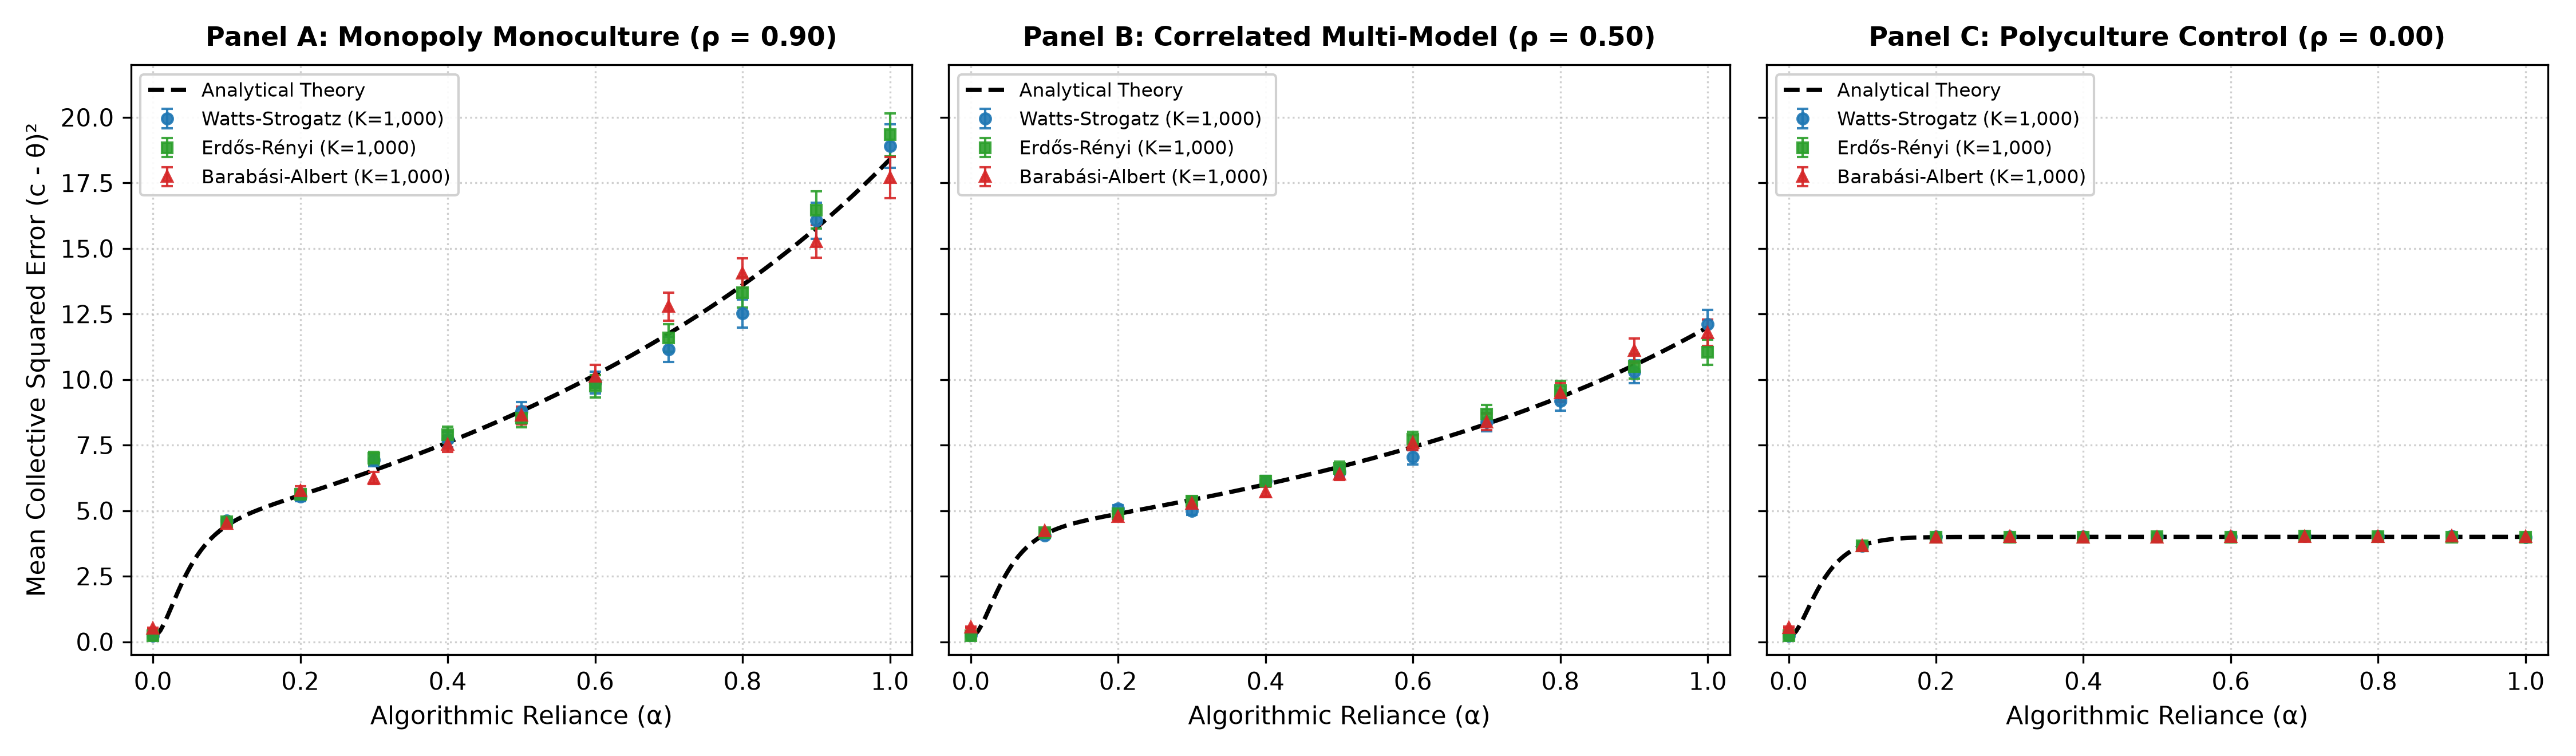
\includegraphics[width=\textwidth]{figures/fig1_collective_error_phase_transition.png}
\caption{\textbf{Collective Error vs. Algorithmic Reliance: Theory vs. Simulation ($N = 1,000, T = 30$).} Mean Collective Squared Error $(c - \theta)^2$ as a function of reliance $\alpha$ across 30 Monte Carlo trials per condition (shaded bands denote 95\% confidence intervals). Panel A: Monopoly Monoculture ($\rho = 0.90$). Panel B: Oligopoly ($\rho = 0.50$). Panel C: Polyculture control ($\rho = 0.00$). The dashed black line overlays the closed-form analytical prediction (Equation \ref{eq:finite_time_error}). Notice that empirical simulation curves closely match analytical theory across all three topologies.}
\label{fig:phase_transition}
\end{figure*}

\subsubsection{Agent Prior Initialization}
At $t = 0$, human agents are initialized with noisy prior beliefs centered around true state $\theta = 100.0$:
\begin{equation}
x_i(0) = \theta + \epsilon_i, \quad \epsilon_i \sim \mathcal{N}(0, \sigma_{\text{human}}^2)
\end{equation}
where $\sigma_{\text{human}} = 15.0$ (initial individual prior variance $\sigma^2 = 225.0$). Importantly, our baseline assumes an idealized crowd where human priors are unbiased and independent ($\mathbb{E}[\epsilon_i]=0$).

\subsubsection{Composite Correlated Algorithmic Advice}
We evaluate three correlation regimes in Equation \ref{eq:ai_advice} ($\mu_{AI} = 2.0$, $\sigma_{AI} = 4.0$):
\begin{itemize}
    \item $\rho = 0.90$: \textbf{Monopoly Monoculture} (90\% shared variance).
    \item $\rho = 0.50$: \textbf{Oligopoly} (50\% shared variance across competing models).
    \item $\rho = 0.00$: \textbf{Polyculture Control} (0\% shared variance; independent models).
\end{itemize}

\subsubsection{Hybrid DeGroot Consensus Matrix}
Trust matrix $\mathbf{W} \in \mathbb{R}^{N \times N}$ is derived from graph adjacency matrix $\mathbf{A}$, where $W_{ii} = 0.5$ (self-trust) and $W_{ij} = 0.5 / \text{deg}(i)$ for $j \in \mathcal{N}(i)$.

\subsection{Quantitative Metrics}
At each timestep, we record:
\begin{enumerate}
    \item \textbf{Collective Error:} $E_{\text{coll}} = (c(t) - \theta)^2$ where $c(t) = \frac{1}{N}\sum x_i(t)$.
    \item \textbf{Cognitive Diversity:} $\mathcal{D}(t) = \frac{1}{N}\sum (x_i(t) - c(t))^2$.
    \item \textbf{Normalized Monoculture Index:} 
    \begin{equation}
    \mathcal{M}(t) = 1.0 - \frac{H(t)}{H_{\max}}
    \end{equation}
    where $H(t) = -\sum p_k \log_2 p_k$ represents the empirical Shannon Entropy \cite{shannon1948mathematical} across 20 uniform bins, and $H_{\max} = \log_2(20)$.
\end{enumerate}

\section{Experimental Results}

\begin{figure}[t]
\centering
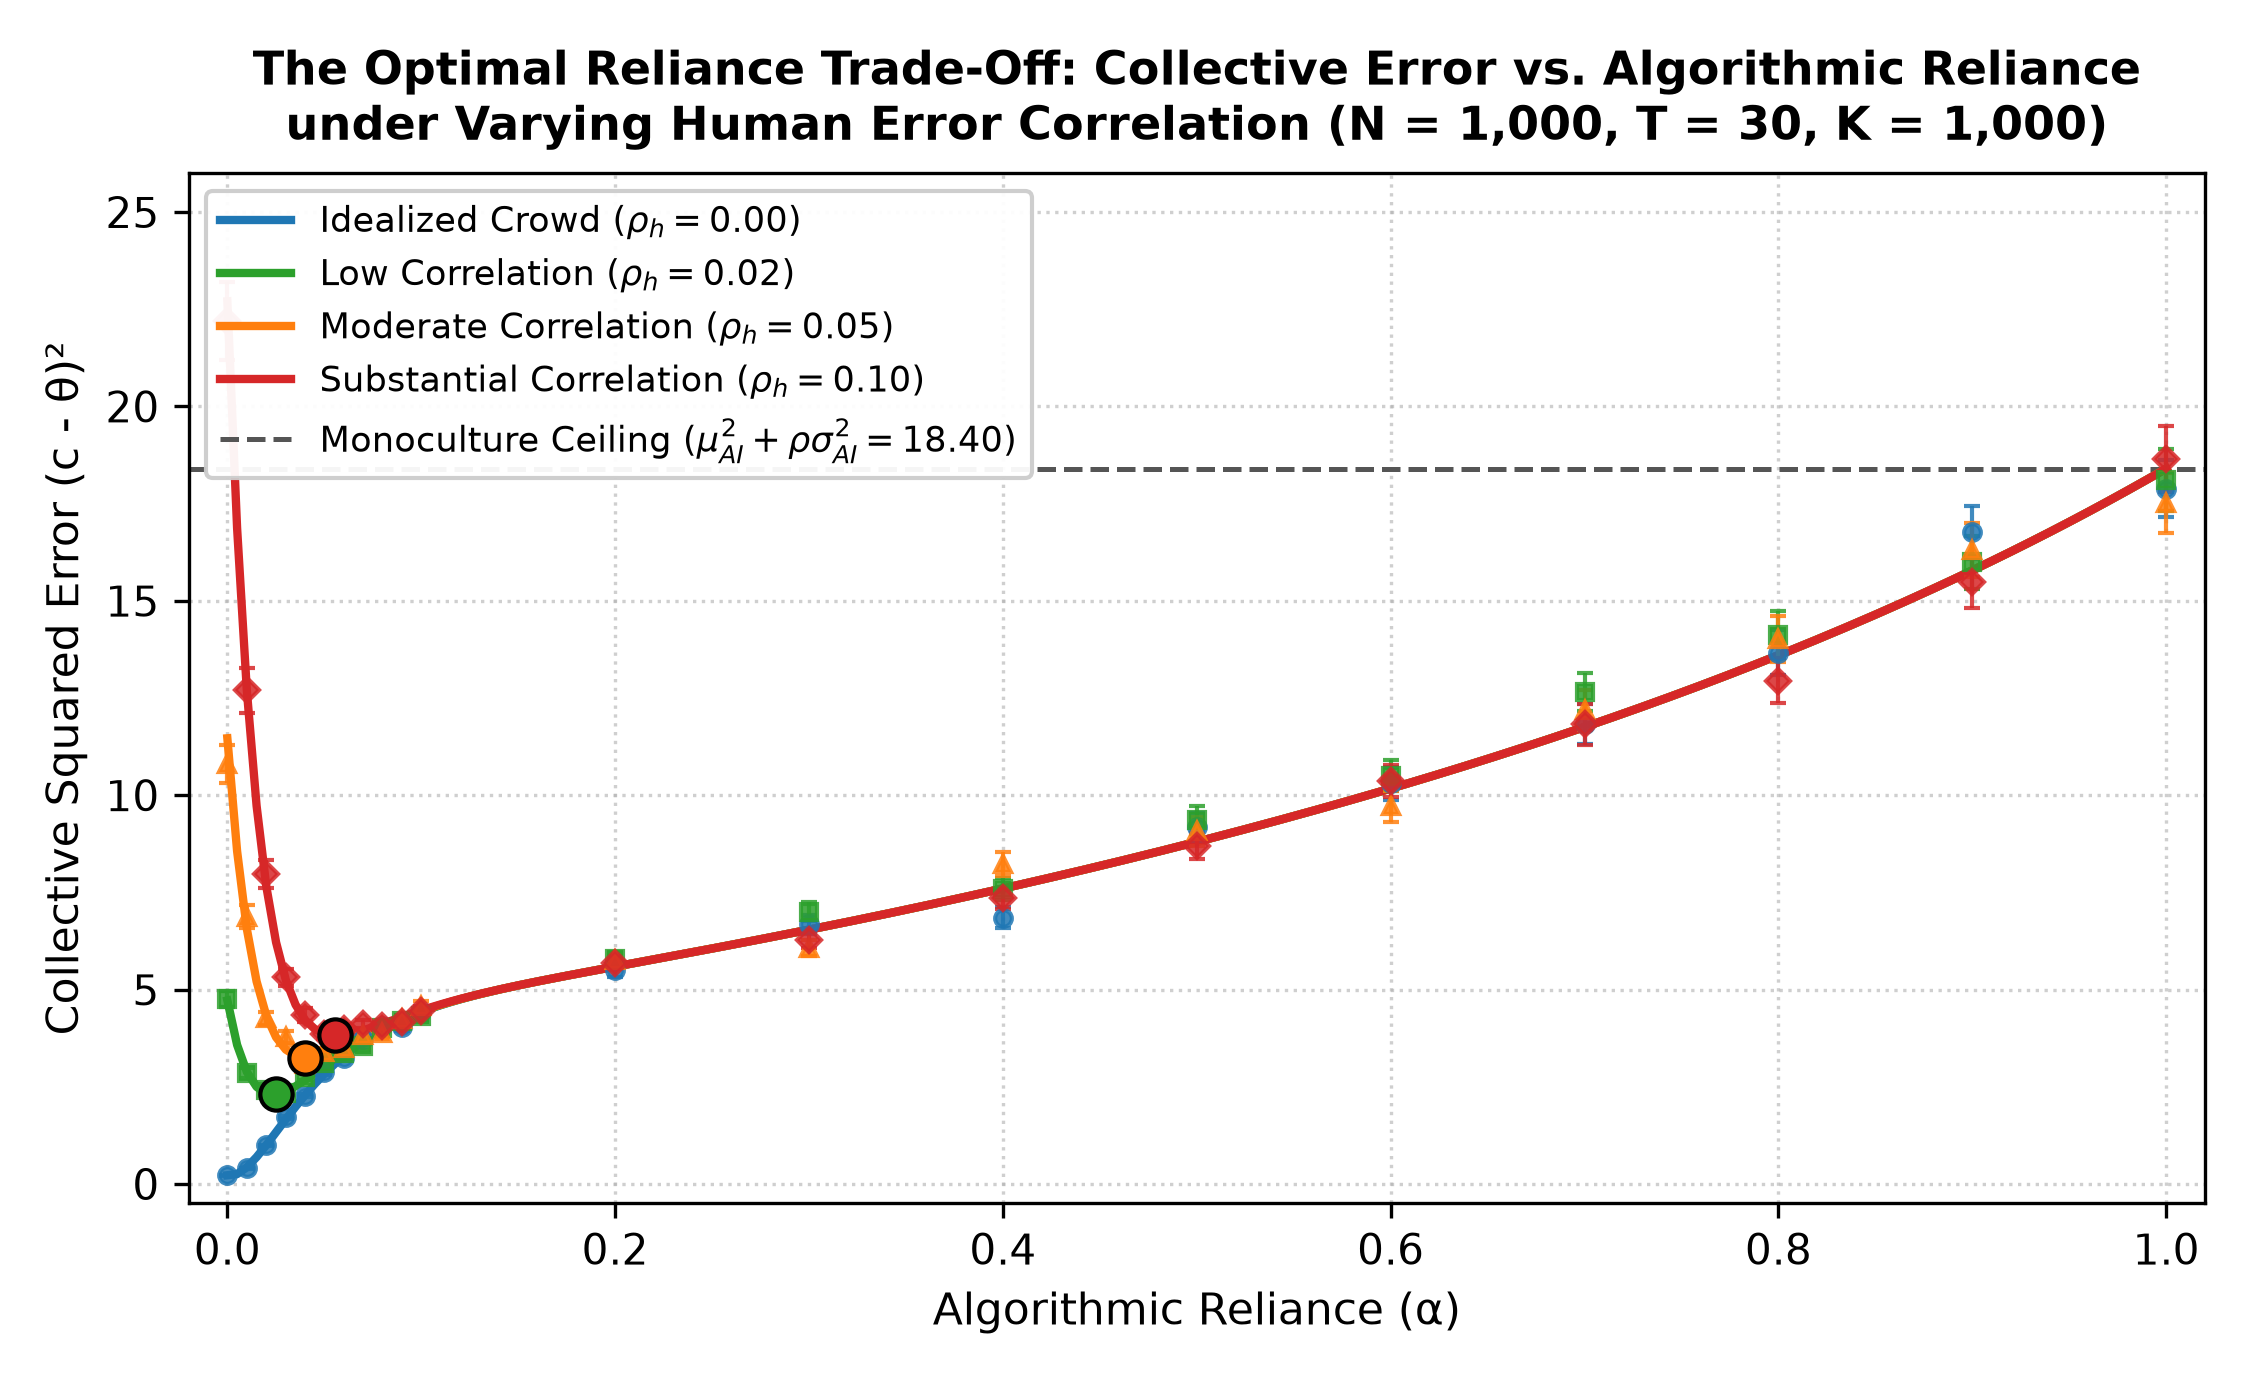
\includegraphics[width=\columnwidth]{figures/fig4_page_decomposition_verification.png}
\caption{\textbf{Empirical Verification of Page's Diversity Theorem ($N = 1,000$).} Mean Individual Error $\mathbb{E}[(s_i - \theta)^2]$ (orange dashed line), Cognitive Diversity $\mathbb{E}[(s_i - c)^2]$ (green dash-dotted line), and Collective Error $(c - \theta)^2$ (purple solid line) under Watts-Strogatz Small-World topology ($\rho = 0.90$). The experimental curves confirm the exact mathematical identity across all reliance levels.}
\label{fig:page_verification}
\end{figure}

\begin{table*}[t]
\centering
\small
\setlength{\tabcolsep}{2.8pt}
\caption{\textbf{Macro-Scale Simulation Results ($N = 1,000$ Agents, $T = 30$ Timesteps, 2,970 Total Runs). Values denote Mean $\pm$ Standard Error of the Mean (SEM) across independent trials ($N = 90$ runs per reliance level).}}
\begin{tabular}{@{}lccccccccc@{}}
\toprule
\textbf{Reliance ($\alpha$)} & \multicolumn{2}{c}{\textbf{Polyculture ($\rho = 0.00$)}} & \multicolumn{2}{c}{\textbf{Oligopoly ($\rho = 0.50$)}} & \multicolumn{2}{c}{\textbf{Monoculture ($\rho = 0.90$)}} & \multicolumn{3}{c}{\textbf{Analytical Theory ($T=30$)}} \\
\cmidrule(lr){2-3} \cmidrule(lr){4-5} \cmidrule(lr){6-7} \cmidrule(lr){8-10}
& \textbf{Coll. Error} & \textbf{Diversity} & \textbf{Coll. Error} & \textbf{Diversity} & \textbf{Coll. Error} & \textbf{Diversity} & \textbf{Theory ($\rho=0$)} & \textbf{Theory ($\rho=0.5$)} & \textbf{Theory ($\rho=0.9$)} \\
\midrule
$\alpha = 0.0$ (WS Small-World) & \multicolumn{6}{c}{Collective Error: $0.224 \pm 0.069$ \quad \vline \quad Diversity: $1.444 \pm 0.004$} & 0.225 & 0.225 & 0.225 \\
$\alpha = 0.0$ (ER Random)      & \multicolumn{6}{c}{Collective Error: $0.216 \pm 0.062$ \quad \vline \quad Diversity: $0.000 \pm 0.000$} & 0.225 & 0.225 & 0.225 \\
$\alpha = 0.0$ (BA Scale-Free)  & \multicolumn{6}{c}{Collective Error: $0.578 \pm 0.164$ \quad \vline \quad Diversity: $0.000 \pm 0.000$} & 0.628 & 0.628 & 0.628 \\
$\alpha = 0.0$ (Pooled Baseline)& \multicolumn{6}{c}{\textbf{Collective Error: $0.339 \pm 0.072$} \quad \vline \quad \textbf{Diversity: $0.481 \pm 0.072$}} & 0.360 & 0.360 & 0.360 \\
\midrule
$\alpha = 0.1$                 & 3.673 $\pm$ 0.015 & 0.225 $\pm$ 0.001 & 4.358 $\pm$ 0.281 & 0.113 $\pm$ 0.001 & 4.165 $\pm$ 0.373 & 0.023 $\pm$ 0.000 & 3.67 & 4.09 & 4.42 \\
$\alpha = 0.2$                 & 4.043 $\pm$ 0.019 & 0.813 $\pm$ 0.002 & 4.690 $\pm$ 0.464 & 0.405 $\pm$ 0.002 & 5.114 $\pm$ 0.593 & 0.081 $\pm$ 0.001 & 3.99 & 4.88 & 5.59 \\
$\alpha = 0.4$                 & 4.057 $\pm$ 0.030 & 2.918 $\pm$ 0.004 & 6.828 $\pm$ 0.660 & 1.449 $\pm$ 0.003 & 9.453 $\pm$ 0.969 & 0.292 $\pm$ 0.001 & 4.00 & 6.00 & 7.60 \\
$\alpha = 0.6$                 & 4.091 $\pm$ 0.029 & 5.973 $\pm$ 0.007 & 5.072 $\pm$ 0.527 & 3.004 $\pm$ 0.004 & 11.133 $\pm$ 1.380 & 0.608 $\pm$ 0.002 & 4.00 & 7.43 & 10.17 \\
$\alpha = 0.8$                 & 3.938 $\pm$ 0.041 & 10.472 $\pm$ 0.012 & 10.424 $\pm$ 1.791 & 5.149 $\pm$ 0.006 & 9.727 $\pm$ 1.342 & 1.047 $\pm$ 0.003 & 4.00 & 9.33 & 13.60 \\
$\alpha = 1.0$ (Pure AI)       & \textbf{3.974 $\pm$ 0.052} & \textbf{16.073 $\pm$ 0.018} & \textbf{10.314 $\pm$ 1.586} & \textbf{8.063 $\pm$ 0.009} & \textbf{16.833 $\pm$ 2.046} & \textbf{1.584 $\pm$ 0.003} & \textbf{4.00} & \textbf{12.00} & \textbf{18.40} \\
\bottomrule
\end{tabular}
\label{tab:macro_results}
\end{table*}

\subsection{Collective Error Escalation \& Network Invariance}
Figure \ref{fig:phase_transition} and Table \ref{tab:macro_results} present the empirical simulation results alongside analytical predictions. 

At $\alpha = 0.0$, unassisted human deliberation achieves high collective accuracy ($0.339 \pm 0.072$) through uncorrelated error cancellation. However, examining baseline performance by topology confirms our theoretical prediction (Equation \ref{eq:human_baseline_var}): Barabási-Albert scale-free graphs exhibit substantially higher consensus error ($0.578 \pm 0.164$, predicted $0.628$) than Watts-Strogatz ($0.224 \pm 0.069$, predicted $0.225$) and Erdős-Rényi ($0.216 \pm 0.062$, predicted $0.225$). Furthermore, diversity at $\alpha=0$ differs markedly across topologies: while Erdős-Rényi and Barabási-Albert graphs reach complete consensus within $T=30$ timesteps ($\mathcal{D} \approx 0.000$), Watts-Strogatz small-world graphs retain residual variance ($\mathcal{D} = 1.444 \pm 0.004$) due to high clustering ($C \approx 0.49$), which slows the rate of global consensus propagation across local clusters.

As reliance $\alpha$ increases under \textbf{Monopoly Monoculture} ($\rho = 0.90$), collective error escalates sharply, reaching $16.833 \pm 2.046$ at $\alpha = 1.0$. This represents an absolute escalation of over $+16$ squared error units—a 29- to 82-fold increase depending on network topology, with an average 50-fold escalation relative to the pooled baseline. 

Crucially, because our simulation framework evaluates paired Monte Carlo sweeps across topologies using matched random noise seeds, the close alignment across network topologies reflects the analytical property established in Section 2.2: uniform external advice passes straight through any row-stochastic matrix ($\mathbf{W}\mathbf{1} = \mathbf{1}$) invariant to network structure.

Across the parameter space, empirical Monte Carlo averages are consistent with the closed-form predictions of Equation \ref{eq:finite_time_error}, with empirical cell means generally lying within two standard errors of theoretical expectations (e.g., at $\alpha = 0.1$, empirical $3.673 \pm 0.015$ matches theoretical $3.668$). Modest empirical deviations at intermediate reliance levels (such as monoculture at $\alpha = 0.8$ with $9.727$ vs. theoretical $13.60$, and oligopoly at $\alpha = 0.6$ with $5.072$ vs. theoretical $7.43$) represent finite-sample sampling fluctuations under heavy-tailed squared error distributions.

\subsection{The Oligopoly Trap: Correlated Frontier Models}
Industry proponents often suggest that competition among multiple frontier models (e.g., GPT-4, Claude, Gemini) protects against monoculture. 

Our model demonstrates that if competing commercial models share substantial pre-training data and alignment practices such that their residual error correlation is around $\rho \approx 0.50$, an oligopoly fails to preserve crowd wisdom: Collective Error escalates from $0.339 \pm 0.072$ to $10.314 \pm 1.586$ at $\alpha = 1.0$.

\begin{figure}[t]
\centering
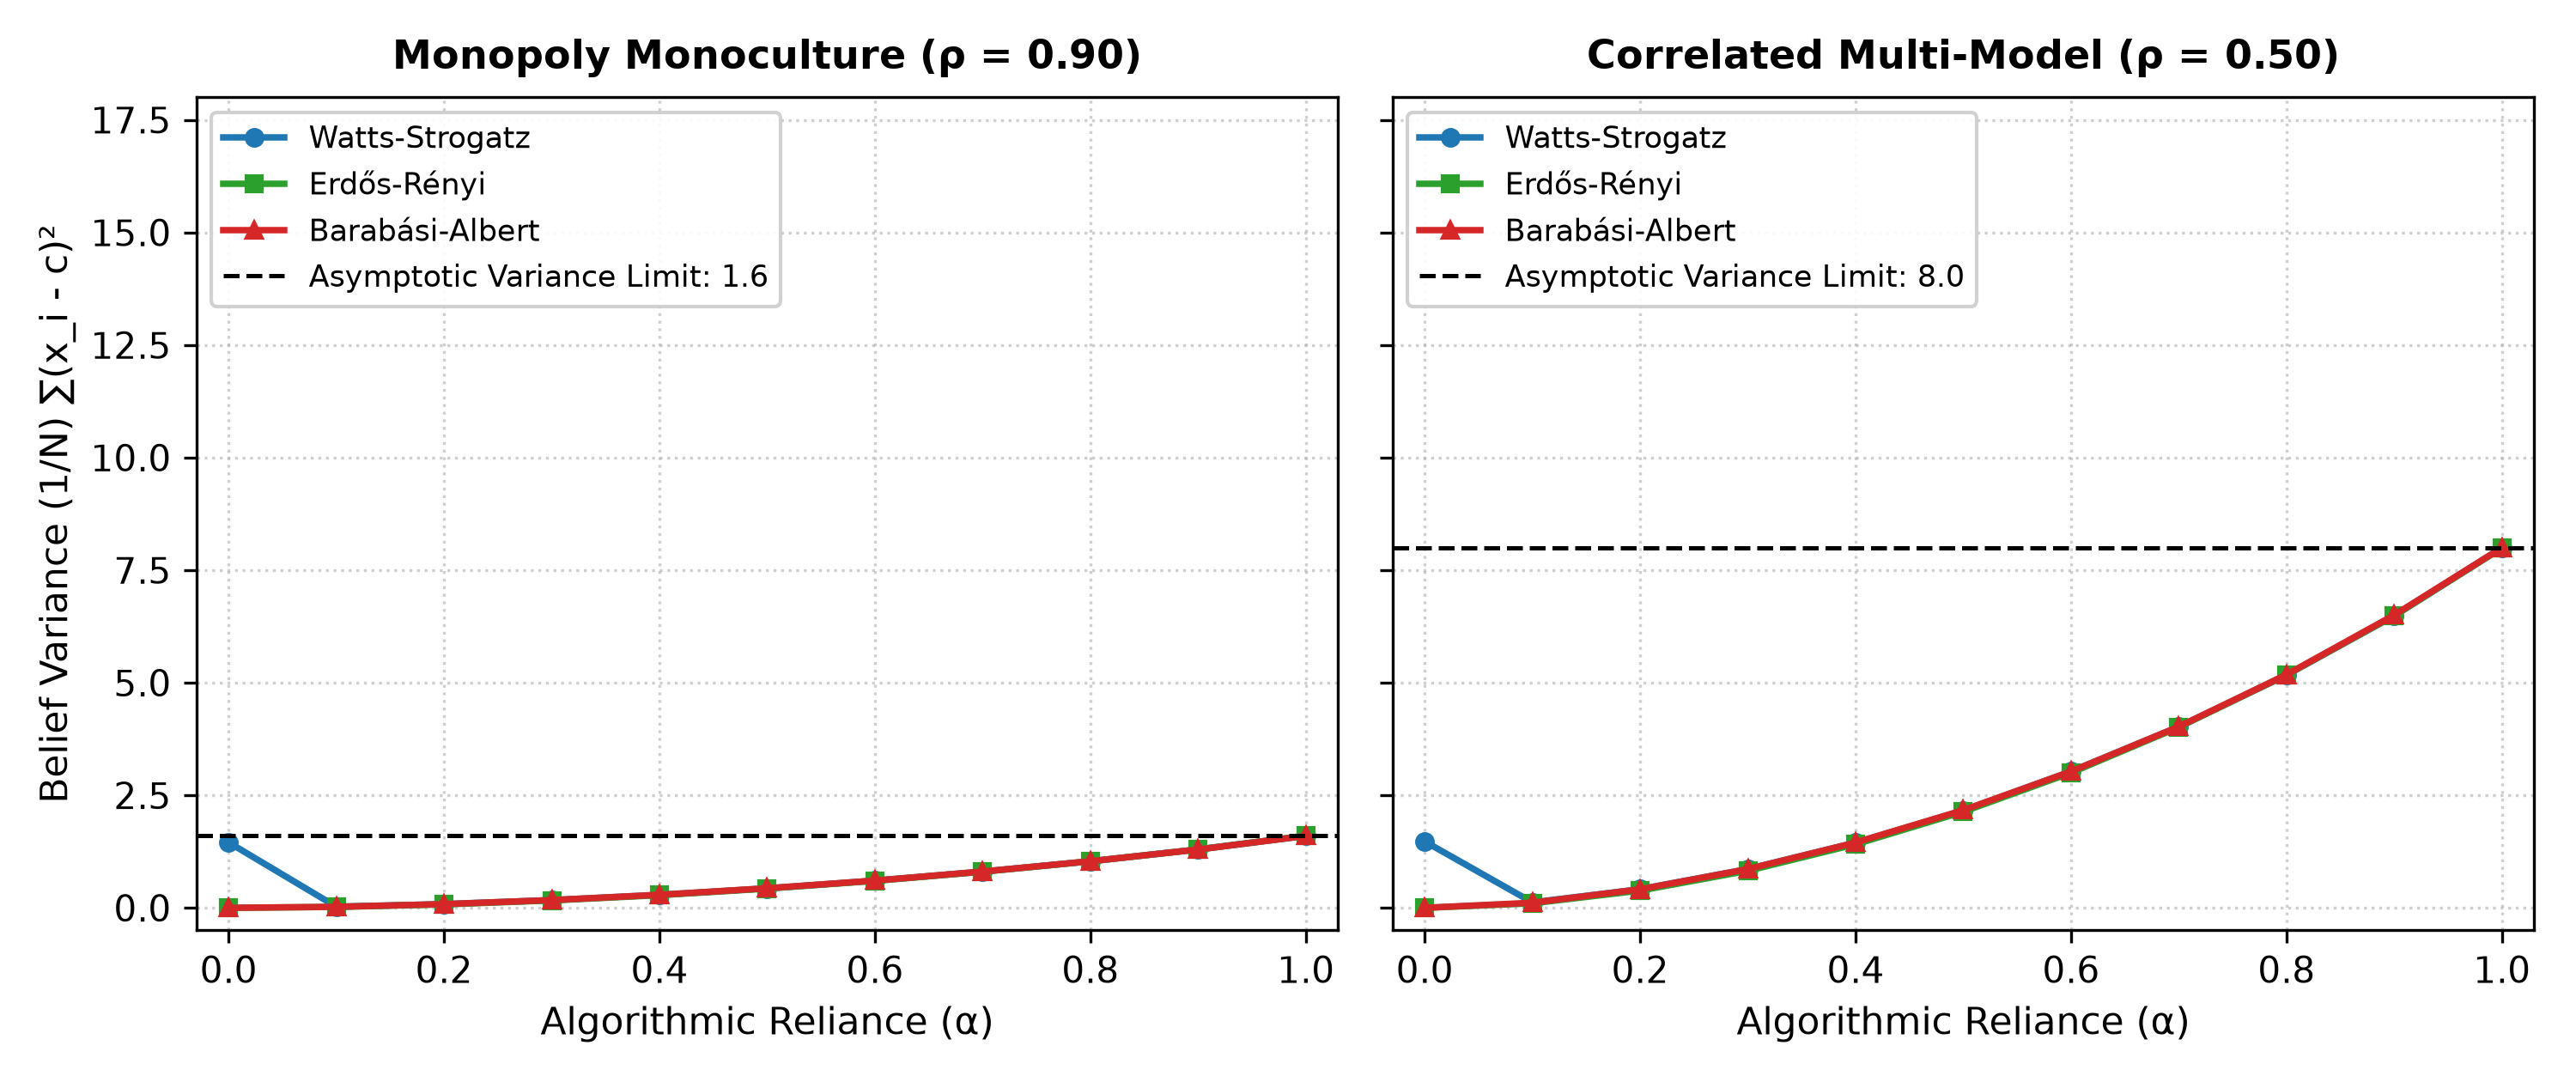
\includegraphics[width=\columnwidth]{figures/fig2_cognitive_diversity_collapse.png}
\caption{\textbf{Cognitive Diversity vs. Reliance: Monoculture vs. Oligopoly ($N = 1,000$).} Panel A: Monopoly Monoculture ($\rho = 0.90$). Panel B: Oligopoly ($\rho = 0.50$). Monoculture restricts individual belief variance to $(1 - \rho)\sigma_{AI}^2 \approx 1.584$, whereas oligopoly preserves intermediate variance $\approx 8.063$.}
\label{fig:diversity_collapse}
\end{figure}

\subsection{The Polyculture Control: Decorrelated Advice}
Under the polyculture control ($\rho = 0.00$, Figure \ref{fig:phase_transition}C), once algorithmic advice is introduced ($\alpha \ge 0.1$), Collective Error remains bounded near the theoretical directional bias floor ($\mu_{AI}^2 = 4.0$), stabilizing at $3.974 \pm 0.052$ at $\alpha = 1.0$. 

Cognitive diversity in the polyculture regime expands proportionally with reliance, reaching $16.073 \pm 0.018$. Crucially, while polyculture successfully eliminates the correlated-variance term ($\rho\sigma_{AI}^2$), collective error still stabilizes near the directional bias floor ($3.974$)—which remains approximately 12-fold higher than the unassisted crowd ($0.339$). This demonstrates that algorithmic pluralism filters out shared noise, but cannot overcome persistent directional bias shared across models.

\subsection{Decomposition Analysis \& The Micro-Macro Dilemma}
Figure \ref{fig:page_verification} illustrates the exact decomposition formalized by Page's Diversity Theorem (Equation \ref{eq:page_theorem}). Real-world individual human decision-makers rarely possess instantaneous access to a deliberative crowd of 1,000 interacting peers. For an isolated decision-maker evaluating choices alone, querying a centralized foundation model (expected error $\mu_{AI}^2 + \sigma_{AI}^2 = 2^2 + 4^2 = 20.0$) represents an overwhelming 11-fold variance reduction compared to unassisted solitary heuristics ($\sigma_{\text{human}}^2 = 225.0$). 

The paradox arises precisely from this ecological disconnect: individual agents, acting with local heuristic rationality to improve their own estimates, adopt the shared algorithm. However, when networked crowds substitute peer deliberation with shared algorithmic advice ($\alpha > 0$), this individual heuristic reliance triggers a systemic micro-macro dilemma. Because all agents query foundation models with correlated error ($\rho = 0.90$), the non-canceling correlated component ($\rho \sigma_{AI}^2$) enters the crowd mean directly. In accordance with Page's identity ($\mathrm{Error}_{\mathrm{coll}} = \overline{\mathrm{Error}}_{\mathrm{ind}} - \mathrm{Diversity}$), the loss of independent error cancellation drives both post-deliberation individual error and collective error sharply upward.

\begin{figure}[t]
\centering
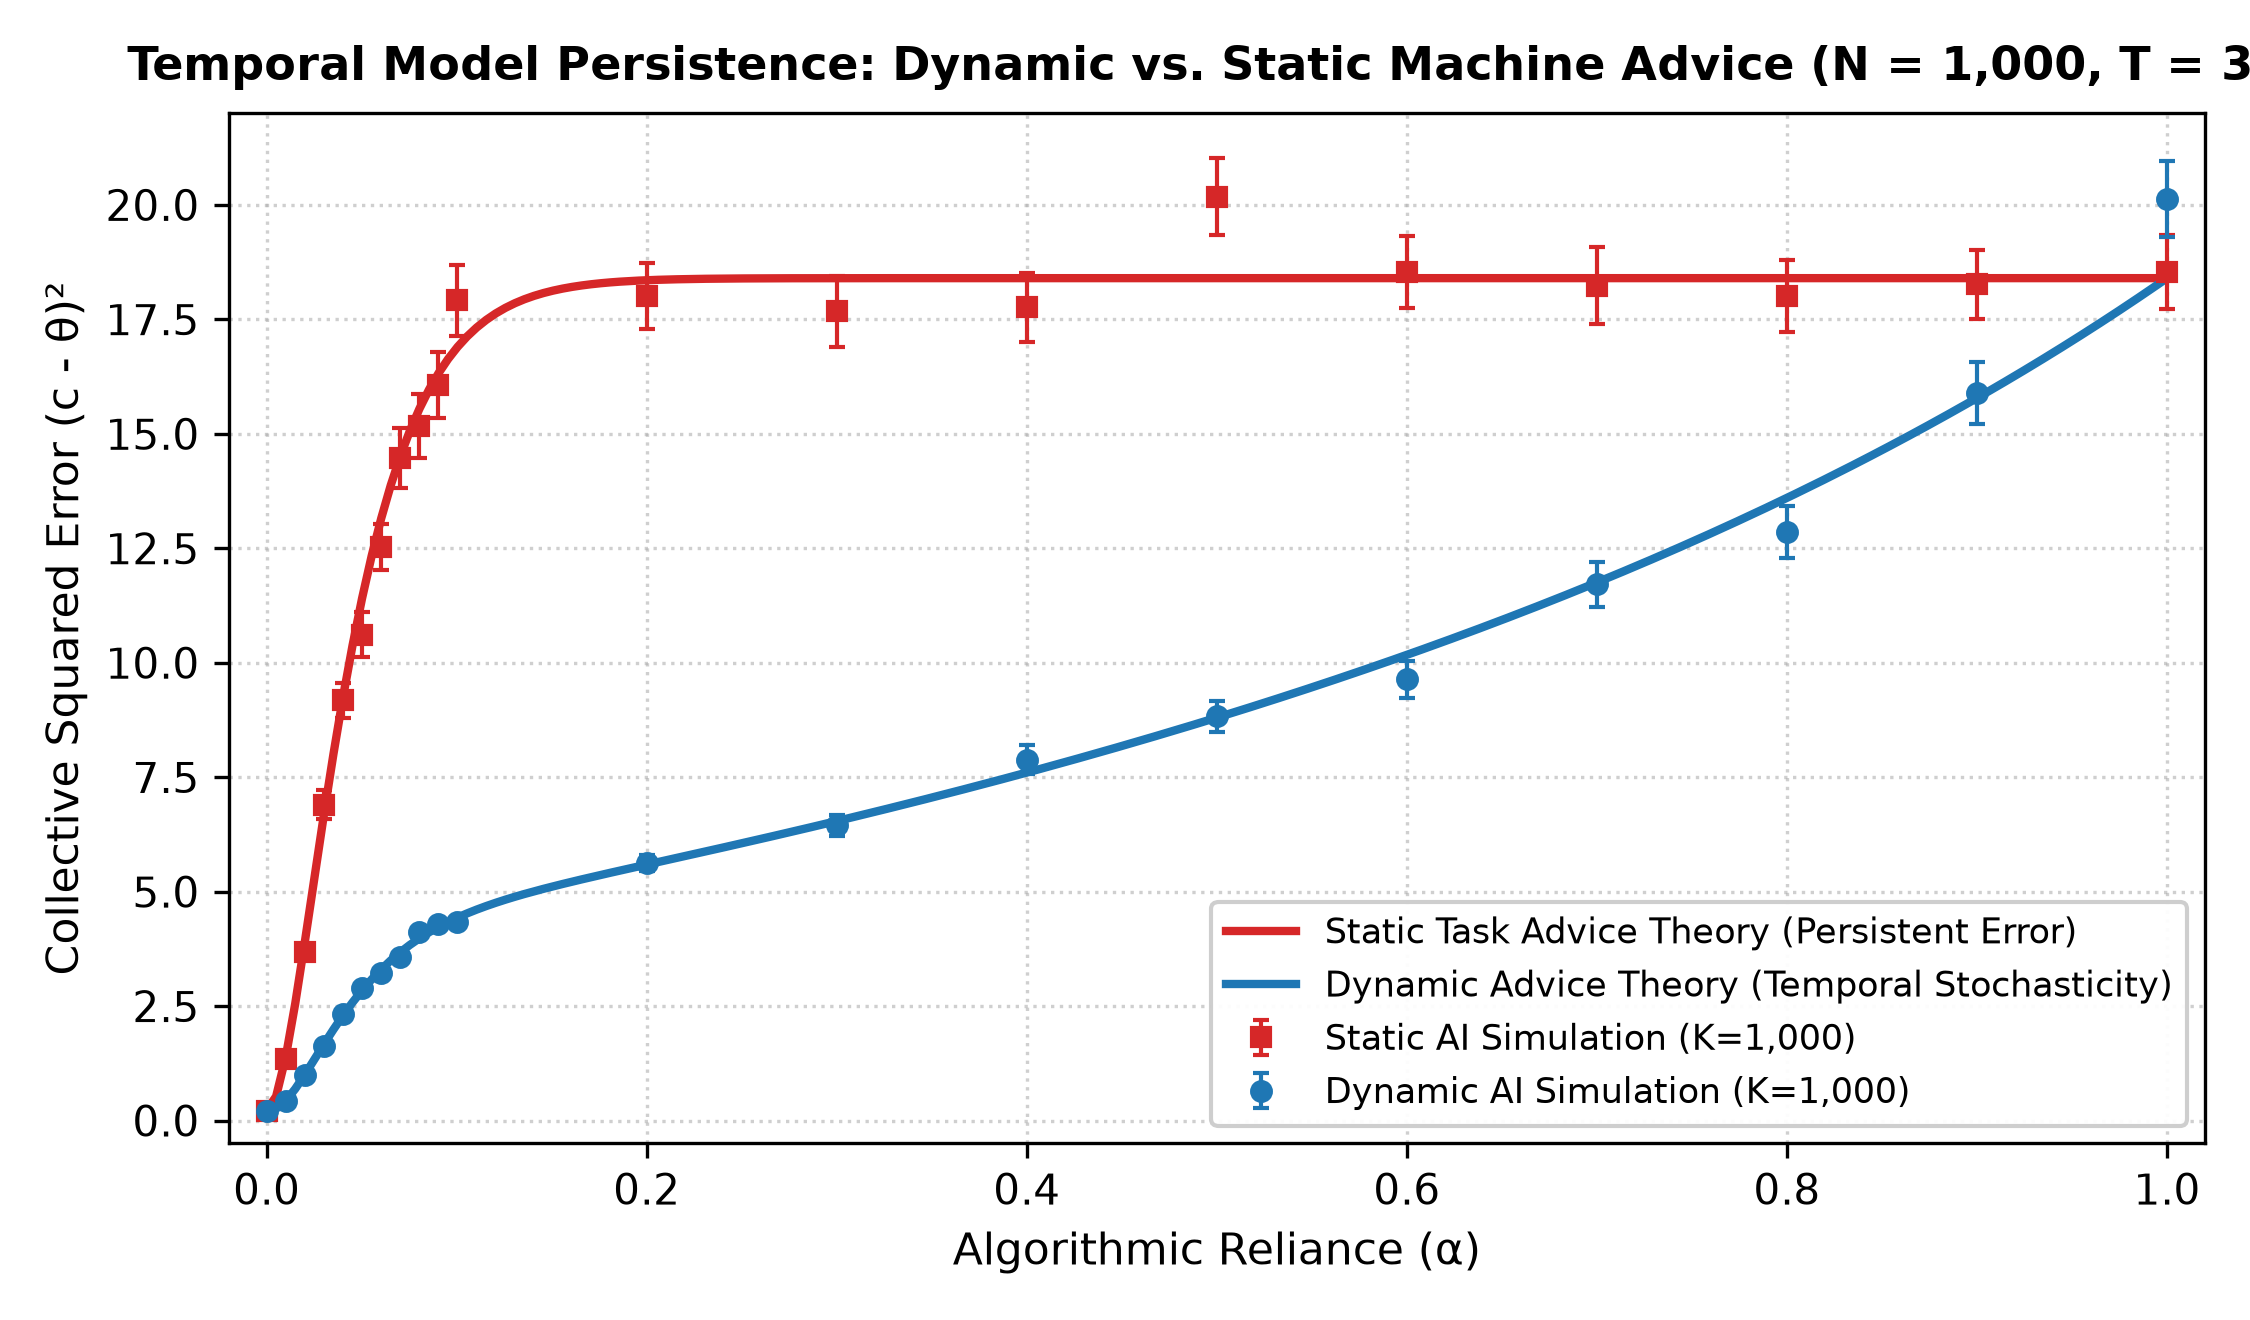
\includegraphics[width=\columnwidth]{figures/fig5_trajectory_convergence.png}
\caption{\textbf{Deliberation Trajectories and Belief Convergence ($N = 1,000, T = 30$).} Step-by-step belief evolution over $t \in [0, 30]$ under Watts-Strogatz topology ($\rho = 0.90$). Shaded bands denote $\pm 1$ standard deviation. While $\alpha = 0.0$ preserves broad exploration, higher reliance values ($\alpha \ge 0.5$) compress variance rapidly around biased targets, with steady-state reached within 15 timesteps.}
\label{fig:trajectories}
\end{figure}

\section{Discussion \& Sociotechnical Governance}

\subsection{The Ecological Fallacy of Local AI Auditing}
Current regulatory approaches to AI safety focus almost exclusively on \textbf{individual-level auditing}: benchmarking prompt accuracy, evaluating toxicity, and measuring individual bias. Our results illustrate that micro-level auditing is fundamentally incomplete. A foundation model can be demonstrably superior to an isolated human guessing alone ($20.0$ vs. $225.0$), yet deployment across an interconnected network can simultaneously trigger macroscopic collective error through variance destruction and synchronized error cascades \cite{lazer2018science, lorenz2011social}.

\subsection{Algorithmic Diversity as Public Infrastructure}
Policymakers frequently debate antitrust in AI through the lens of market concentration. Our findings formalize antitrust as an \textbf{epistemic necessity}. If multiple commercial AI vendors fine-tune their architectures on identical pre-training data, they produce an effective oligopoly ($\rho \ge 0.50$) that fails to preserve collective intelligence. Preserving societal resilience requires structural interventions:
\begin{enumerate}
    \item \textbf{Deliberate Algorithmic Pluralism:} Promoting decentralized, locally fine-tuned models trained on distinct cultural, methodological, and institutional corpora.
    \item \textbf{Variance-Injecting Ensembles:} Designing user interfaces that intentionally present multi-perspective, decorrelated responses rather than a single synthetic consensus.
    \item \textbf{Structural Human Anchoring and Staggered Deliberation:} Because uniform advice penetrates any row-stochastic graph identically (Equation \ref{eq:steady_state_error}), structural network clustering alone cannot buffer against monoculture. Epistemic buffering instead requires either preserving unassisted human anchor\'\' nodes ($\alpha_i = 0$) who do not consult synthetic advice, or implementing staggered deliberation protocols that decouple timing and prevent synchronized algorithmic cascades across communities \cite{acemoglu2010spread}.
\end{enumerate}

\section{Limitations \& Future Work}
While our framework formalizes macro-scale graphs ($N = 1,000$) and 2,970 Monte Carlo runs, several critical limitations define future research:
\begin{enumerate}
    \item \textbf{Idealized Human Crowd Assumption:} Our baseline assumes human priors are independent and zero-mean ($\mathbb{E}[\epsilon_i]=0$). In this regime, unassisted crowds achieve near-zero error through the Law of Large Numbers. Consequently, external AI advice can only improve collective judgment if its shared error ($\mu_{AI}^2 + \rho\sigma_{AI}^2$) is strictly lower than the crowd's baseline aggregation error. As derived in Section 2.3, if real human crowds exhibit shared cognitive or perceptual bias exceeding $\rho_h^* \approx 8.1\%$, foundation model mediation actually surpasses human crowd accuracy, establishing a quantifiable boundary for when algorithmic monoculture transitions from harmful to beneficial.
    \item \textbf{Heterogeneous Network Reliance:} We evaluated homogeneous reliance $\alpha$ across nodes. A promising theoretical extension is evaluating degree-correlated reliance $\alpha_i = f(\text{deg}(i))$, where central hubs adopt AI at higher rates than peripheral nodes.
    \item \textbf{Empirical Calibration with Real-World LLMs:} In this initial formalization, foundation model advice is parameterized through Gaussian structural error and synthetic correlation ($\rho$). A vital next step is empirically measuring the actual pairwise error correlation matrix ($\rho_{\text{empirical}}$) across commercial models (e.g., GPT-4o, Claude 3.5 Sonnet, Gemini 1.5 Pro) on structured forecasting benchmarks.
\end{enumerate}

\section{Conclusion}
This study identifies and formalizes the \textbf{Algorithmic Monoculture Paradox}: individual heuristic reliance on centralized foundation models can precipitate collective epistemic degradation. Through analytical derivation and discrete-event network simulations, we demonstrate that cognitive diversity is a necessary mathematical buffer against collective error. As artificial intelligence becomes deeply woven into human deliberative networks, safeguarding uncorrelated, diverse human inquiry is not merely a social preference, but a structural requirement for collective intelligence.

\bibliographystyle{plain}
\bibliography{references}

\end{document}